\subsection{实验目的-了解 iptables 常用的基本命令}
了解 iptables 常用的基本命令.
%
\subsection{实验原理}
iptables 是用来设置、维护和检查 Linux 内核的 IP 包过滤规则的。可以定
义不同的表,每个表都包含几个内部的链,也能包含用户自定义的链。每个链都
是一个规则列表,对对应的包进行匹配:每条规则指定应当如何处理与之相匹配
的包。这被称作 target(目标),也可以跳向同一个表内的用户定义的链。
%
\subsection{实验环境}
操作系统:CentOS 6.5
%
\subsection{实验步骤}
\subsubsection{查看 iptables 使用方法}
一般而言,我们学习某个软件的使用方法,除了在网上或者使用书籍进行
学习,最快捷有效的方式就是直接查看帮助。右键单击桌面,选择``在终端中打开''。
\begin{figure}[H]
  \begin{center}
    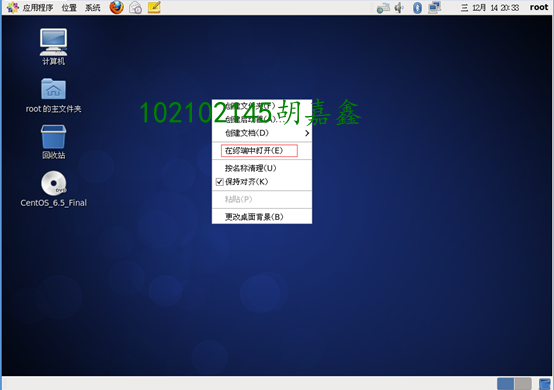
\includegraphics[width=0.50\textwidth]{2_4_1.png}
  \end{center}
\end{figure}

在终端中输入命令
\begin{minted}[bgcolor=bg]{sh}
iptables -h
\end{minted}
则会列出 iptables 的使用方法。
若想要看 iptables 更加详细的使用方法,可以使用命令
\begin{minted}[bgcolor=bg]{sh}
man iptables
\end{minted}
%
\subsubsection{iptables 基本命令}
iptables 命令的通用格式为:
\begin{minted}[bgcolor=bg,breaklines=true]{sh}
iptables [-t tables] COMMAND chain [-m matchname [per-match-options]] -j targetname [per-target-options]
\end{minted}
其中,tables 包括 filter、nat、mangel 和 raw,
chain 包括 INPUT、OUTPUT、FORWARD、PREROUTING 和 POSTROUTING。
当不指定表时,默认表为 filter。

iptables 命令的使用格式可用图表示如下。
\begin{figure}[H]
  \begin{center}
    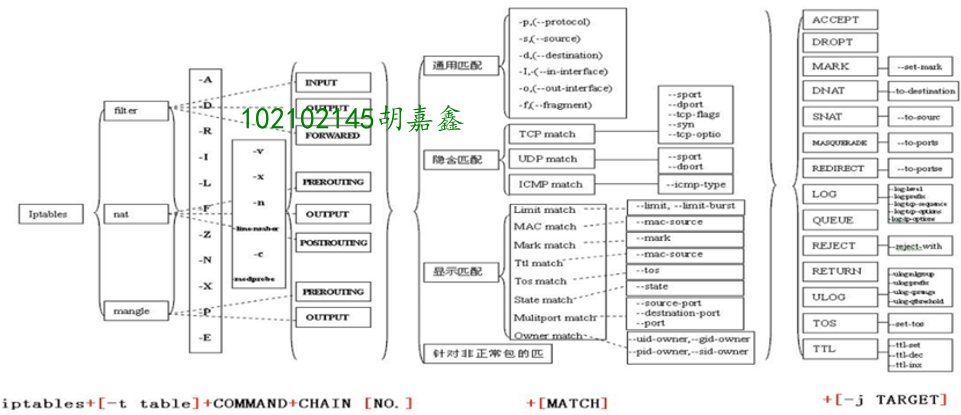
\includegraphics[width=0.50\textwidth]{2_4_2.png}
  \end{center}
\end{figure}

对上图进行简化。
\begin{figure}[H]
  \begin{center}
    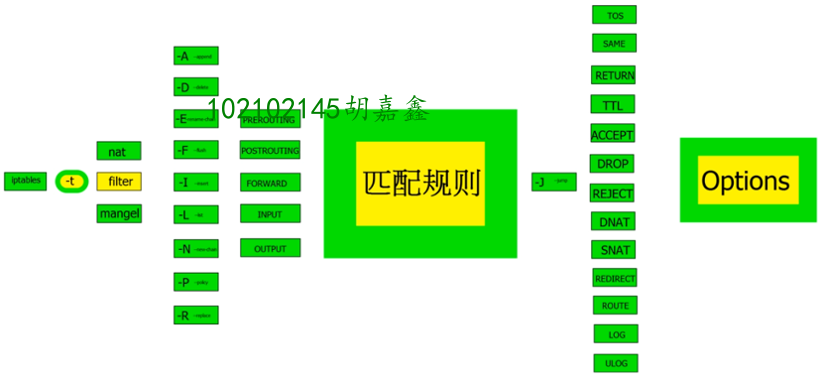
\includegraphics[width=0.50\textwidth]{2_4_3.png}
  \end{center}
\end{figure}

下面对 COMMAND 进行介绍。
\begin{enumerate}
  \item 常见用于链管理的参数有:
    \begin{itemize}
      \item \mintinline{sh}{-N}:new,自定义一条新的规则链
      \item \mintinline{sh}{-X}:delete/drop, 删除自定义的规则链,指明名字删除一个,不指明将删除多个
      \item \mintinline{sh}{-P}:policy,设置默认策略,指明是黑名单还是白名单,对于 filter 表中的链
        而言,其默认策略有 ACCEPT(接受)、DROP(丢弃)和 REJECT(拒绝)
      \item \mintinline{sh}{-E}:重命名自定义链,引用计数不为 0 的自定义链,不能被重命名或者删除
    \end{itemize}
  \item 常见的用于规则管理的参数有:
    \begin{itemize}
      \item \mintinline{sh}{-A}:append,追加规则
      \item \mintinline{sh}{-I}:insert,插入规则,需要指明位置,省略时表示第一条
      \item \mintinline{sh}{-D}:delete,删除规则,指明规则号删除或者指明规则本身
      \item \mintinline{sh}{-R}:replace,替换指定链上的指定规则,指明替换号或者指明替换规则本身
      \item \mintinline{sh}{-F}:flush,清空指定的规则链,指明链,即清空指定链上的规则;不指明链,
        即清空所有链上的规则
      \item \mintinline{sh}{-Z}:zero, 置零,匹配到的报文个数或者匹配到的所有报文的大小之和(字节数)
    \end{itemize}
  \item 查看信息的常用参数有:
    \begin{itemize}
      \item \mintinline{sh}{-L}:必选,list,列出指定链上的所有规则,下面的几个为附加子参数
      \item \mintinline{sh}{-n}:numberic,以数据格式显示地址和端口
      \item \mintinline{sh}{-v}:verbose,详细信息,vv 或者 vvv(v 的个数越多越详细)
      \item \mintinline{sh}{-x}:exactly(精确的),显示计数器结果的精确值
      \item \mintinline{sh}{--line-numbers}:显示规则的序号
    \end{itemize}
\end{enumerate}

下面对匹配条件进行介绍。
\begin{enumerate}
  \item  基本匹配条件:无需加载任何模块,由 iptables/netfilter 自行提供
    \begin{itemize}
      \item \mintinline{sh}{-s,--source address[/mask][,...]}:检查报文中源 IP 地址, 是否符合此处指
        定的地址或范围
      \item \mintinline{sh}{-d,--destination address[/mask][,...]}:检查报文中的目标 IP 地址,是否符
        合此处指定的地址或范围
      \item \mintinline{sh}{-p,--protocol protocol}:表明在传输层应用的协议,其可以有 tcp,udp,udplite,
        icmp,icmpv6,esp,ah,sctp,mh 或者 all(包括 tcp、udp 和 icmp 3 个)
      \item \mintinline{sh}{-i,--in-interface name}:
        只能应用于数据报文流入的接口,作用于链 INPUT,FORWARD 和 PREROUTING
      \item \mintinline{sh}{-o,--out-interface name}:只能应用于数据报文流出的接口, 作用于链 OUTPUT,
        FORWARD 和 POSTROUTING
    \end{itemize}
  \item  隐匿扩展:不需要手动加载扩展模块,因为它们是对协议的扩展,所以但凡使
    用 \mintinline{sh}{-p} 指明了协议,就表示已经指明了要扩展的模块
    \begin{itemize}
      \item tcp 协议:
        \begin{enumerate}
          \item \mintinline{sh}{--source-port,--sport port[:port]}:匹配报文的源端口,可以是端口范围
          \item \mintinline{sh}{--destination-port,--dport port[:port]}:匹配报文的目标端口,可以是端口范围
          \item \mintinline{sh}{--tcp-flags mask comp}:mask 为必须要检查的标识位,必须以逗号分隔;comp
            必须为 1 的标识位,必须以逗号分隔
          \item \mintinline{sh}{--syn}:匹配第一次握手
        \end{enumerate}
      \item udp 协议:
        \begin{enumerate}
          \item \mintinline{sh}{--source-port,--sport port[:port]}: 匹配报文的源端口,可以是端口范围
          \item \mintinline{sh}{--destination-port,--dport port[:port]}:匹配报文的目标端口,可以是端口范围
        \end{enumerate}
      \item icmp 协议:\mintinline{sh}{--icmp {type[/code] | typename}}
    \end{itemize}
  \item  显示扩展:必须使用\mintinline{sh}{-m} 选项手动加载模块,
    其扩展模块路径为: \mintinline{sh}{/lib64/xtables},
    其中大写的为目标扩展,小写的为规则扩展。
  \item multiport 扩展:以离散方式定义多端口匹配,但最多指定 15 个端口
    \begin{enumerate}
      \item \mintinline{sh}{--source-ports,--sports port[,port|,port:port]}:指定多个源端口
      \item \mintinline{sh}{--destination-ports,--dports port[,port|,port:port]}:指定多个源端口
      \item \mintinline{sh}{--ports port[,port|,port:port]}:指定多个目标及源端口
    \end{enumerate}
  \item iprange 扩展:指明连续的(不过一般不能是整个网络)ip 地址范围
    \begin{enumerate}
      \item \mintinline{sh}{--src-range from[-to]}:源 IP 地址
      \item \mintinline{sh}{--dst-range from[-to]}:目标 IP 地址
    \end{enumerate}
  \item connlimit 扩展:对每客户端 IP 做并发连接数量匹配
    \begin{enumerate}
      \item \mintinline{sh}{--connlimit-upto n}:当现在的连接数量低于或等于这个数量(n),就匹配
      \item \mintinline{sh}{--connlimit-above n}:当现有的连接数量大于这个数量, 就匹配
    \end{enumerate}
  \item limit 扩展:基于收发报文的速率做匹配
    \begin{enumerate}
      \item \mintinline{sh}{--limit rate [/second|/minute|/hour]}:平均速率
      \item \mintinline{sh}{--limit-burst NUMBER}:峰值数量,默认 5 个
    \end{enumerate}
  \item state 扩展:根据连接追踪机制,查检连接的状态,
    跟 TCP 没有关系,是内核中 netfilter 实现,
    能实现 tcp,udp,icmp 的连接追踪,
    内核会记录每一个连接(放置在内存中),谁通过什么协议访问什么服务,
    访问的时间,这种机制被称之为 conntrack 机制。
    也正是有了 state 扩展,iptables 成为了有连接追踪的防火墙,
    安全性更高。是由 state 扩展提供,
    库文件为 \mintinline{sh}{ibxt_conntrack.so}。
    追踪连接功能在内核的内存空间中,把出去和进来的连接通过模板建立关联关系.
    追踪本机的请求和响应之间的关系,状态如下几种:
    \begin{enumerate}
      \item NEW:新发起的请求
      \item ESTABLISHED:new 状态之后,连接追踪模板中为其建立的条目失效之前期间内所有的通信状态
      \item RELATED:相关的连接,如 FTP 协议中的命令连接与数据连接之间的关系
      \item INVALID:无效的连接,如 tcp 状态全为 1 或者全为 0 的连接
      \item UNTRACKED:未进行追踪的连接
    \end{enumerate}
    调整连接追踪功能所容纳的最大连接数量:
    \begin{minted}[bgcolor=bg]{sh}
    /proc/sys/net/nf_conntrack_max
    \end{minted}
    已经追踪到的并记录下来的连接:
    \begin{minted}[bgcolor=bg]{sh}
    /porc/net/nf_conntrack
    \end{minted}
    不同协议的连接追踪状态时长(可修改):
    \begin{minted}[bgcolor=bg]{sh}
    /proc/sys/net/netfilter
    \end{minted}
    \mintinline{sh}{--state STATE}:
    多个 state 可以使用逗号分隔.
    iptables 的连接追踪表最大容量为
    \begin{minted}[bgcolor=bg]{sh}
    cat /proc/sys/ipv4/ip_conntrack_max
    \end{minted}
    链接达到各种状态的超时后,会从表中删除,
    当模板满载时,后续的链接可能会超时,可以有如下两种解决方法
    (但加大 max 值, 也会加大内存的压力)
    \begin{enumerate}
      \item 修改 max 的内核参数:
        \begin{minted}[bgcolor=bg]{sh}
        vim /etc/sysctl.conf
        \end{minted}
      \item 降低 \mintinline{sh}{nf_conntrack timout} 时间:
        \begin{minted}[bgcolor=bg]{sh}
        vim /etc/sysctl.conf
        \end{minted}
        放行被动模式的 ftp 服务,
        需手动加载 \mintinline{sh}{nf_conntrack_ftp}:
        \begin{minted}[bgcolor=bg]{sh}
        modprobe nf_conntrack_ftp
        \end{minted}
    \end{enumerate}
\end{enumerate}
%
target 的分类:
\begin{enumerate}
  \item ACCEPT:接受
  \item DROP:丢弃
  \item REJECT:拒绝
  \item RETURN:返回调用链
  \item REDIRECT:端口重定向
  \item LOG:记录日志,\mintinline{sh}{--log-level LEVEL} 用于设置日志的等级,
    \mintinline{sh}{--log-prefix PFREFIX} 用于设置日志的提示语句的前缀
  \item MASK:做防火墙标记
  \item DNAT:目标地址转换
  \item SNAT:源地址转换
  \item MASQUERADE:地址伪装
\end{enumerate}
